\documentclass[12pt,a4paper]{report}  %紙張設定
\usepackage{xeCJK}%中文字體模組
\setCJKmainfont{標楷體} %設定中文字體
%\setCJKmainfont{MoeStandardKai.ttf}
\newfontfamily\sectionef{Times New Roman}%設定英文字體
%\newfontfamily\sectionef{Nimbus Roman}
\usepackage{enumerate}
\usepackage{titlesec}
\titleformat{\chapter}[display]
{\normalfont\fontsize{20}{22}\selectfont\bfseries\filcenter}
{\chaptertitlename\ \thechapter}{10pt}{\fontsize{18}{22}\selectfont}
\titlespacing*{\chapter}{0pt}{-10pt}{2pt}
\usepackage{amsmath,amssymb}%數學公式、符號
\usepackage{amsfonts} %數學簍空的英文字
\usepackage{graphicx, subfigure}%圖形
\usepackage{fontawesome5} %引用icon
\usepackage{type1cm} %調整字體絕對大小
\usepackage{textpos} %設定文字絕對位置
\usepackage[top=2.5truecm,bottom=2.5truecm,
left=3truecm,right=2.5truecm]{geometry}
\usepackage{titlesec} %目錄標題設定模組
\usepackage{titletoc} %目錄內容設定模組
\usepackage{textcomp} %表格設定模組
\usepackage{multirow} %合併行
%\usepackage{multicol} %合併欄
\usepackage{CJK} %中文模組
\usepackage{CJKnumb} %中文數字模組
\usepackage{wallpaper} %浮水印
\usepackage{listings} %引用程式碼
\usepackage{hyperref} %引用url連結
\usepackage{setspace}
\usepackage{lscape}%設定橫式
\lstset{language=Python, %設定語言
		basicstyle=\fontsize{10pt}{2pt}\selectfont, %設定程式內文字體大小
		frame=lines,	%設定程式框架為線
}
%\usepackage{subcaption}%副圖標
\graphicspath{{./../images/}} %圖片預設讀取路徑
\usepackage{indentfirst} %設定開頭縮排模組
\renewcommand{\figurename}{\Large 圖.} %更改圖片標題名稱
\renewcommand{\tablename}{\Large 表.}
\renewcommand{\lstlistingname}{\Large 程式.} %設定程式標示名稱
\hoffset=-5mm %調整左右邊界
\voffset=-8mm %調整上下邊界
\setlength{\parindent}{3em}%設定首行行距縮排
\usepackage{appendix} %附錄
\usepackage{diagbox}%引用表格
\usepackage{multirow}%表格置中

%--------------------封面-----------------------------%
\begin{document}

\begin{center}
\vspace*{1cm}
  \fontsize{18}{16}\selectfont \textbf{POLITECNICO DI TORINO}\par
\end{center}
\begin{center}
    \fontsize{18}{16}\selectfont \textbf{都靈理工大學}\\
\end{center}
% 在图像下方添加分界线
\noindent\rule{\textwidth}{0.4pt}
\vspace{0.5em}
\begin{center}
  \fontsize{12}{16}\selectfont \textbf{ANALYSIS OF THE ODOO SOFTWARE CAPABILITIES REGARDING 
PRODUCT LIFECYCLE MANAGEMENT, MANUFACTURING EXECUTION 
SYSTEMS AND THEIR INTEGRATION}\par
\end{center}
\begin{center}
   \fontsize{12}{22}\selectfont \textbf{ODOO 軟體功能分析產品生命週期管理、製造執行系統及其集成}
\end{center}
\vspace{1em}
\begin{figure}[h]
\vspace{2cm}
    \centering
    
\includegraphics[width=0.33\textwidth]{logo} 
    \label{fig:logo}
\end{figure}
\vspace{2cm}
\noindent
\small\textbf{SUPERVISORS} \hfill \textbf{CANDIDATE}\\
\small\textbf{指導者} \hfill \textbf{申請人}\\
\small\textbf{Giulia Bruno } \hfill \textbf{Lucas Flabiano Perotti}\\
\small\textbf{朱莉婭·布魯諾} \hfill \textbf{盧卡斯·弗拉比亞諾·佩羅蒂}\\
\small\textbf{Franco Lombardi}\hspace{\fill} \\
\small\textbf{佛朗哥·隆巴迪}\hspace{\fill} \\
\noindent\rule{\textwidth}{0.4pt}
\begin{center}
\fontsize{12}{22}\selectfont {Academic Year 2020 – 2021}\\
\fontsize{12}{22}\selectfont {2020 – 2021 學年}
\end{center}
\thispagestyle{empty}
\newpage
%--------------------分頁-----------------------------%
\vspace*{\fill}
\vspace*{\fill}
\begin{raggedright}
    \fontsize{12}{14}\selectfont This work is subject to the Creative Commons Licence\\
    \fontsize{12}{14}\selectfont 本作品受知識共享授權約束\\[2ex]
    \fontsize{12}{12}\selectfont All Rights Reserved\\
    \fontsize{12}{12}\selectfont 版權所有\\

\end{raggedright}
\thispagestyle{empty}
\newpage
%--------------------致謝-----------------------------%
\renewcommand{\baselinestretch}{1.5} %設定行距
\pagenumbering{roman} %設定頁數為羅馬數字
\clearpage  %設定頁數開始編譯
\sectionef
\addcontentsline{toc}{chapter}{ACKNOWLEDGMENTS} %將摘要加入目錄
\begin{center}
\LARGE\textbf{ACKNOWLEDGMENTS}\\
\LARGE\textbf{致謝}\\
\end{center}
\fontsize{14pt}{2.5pt}\sectionef
  {  I would like to thank Dr. Giulia Bruno for her expert advice and invitation to develop this project, as well as Emiliano Traini, for his extraordinary support in this thesis process.}。\\[1pt]

\fontsize{14pt}{5pt}\sectionef
  {  我要感謝朱莉婭·布魯諾博士的專家建議和邀請來開發這個
專案以及埃米利亞諾·特拉尼,感謝他在本論文過程中的非凡支持。}\\[15pt]

\fontsize{14pt}{2.5pt}\sectionef
  {  My most sincere gratitude to my parents, Julio and Michelle, who gave me everything, 
from my life to their extensive and unconditional support and encouragement; also, to my 
brothers and my fiancée Ana, who inspired me through all these years.}\\[1pt]

\fontsize{14pt}{5pt}\sectionef
  {  我最誠摯的感謝我的父母Julio和Michelle,他們給了我一切,從我的生活到他們廣泛、無條件的支持和鼓勵; 還有,對我的
兄弟們和我的未婚妻安娜這些年來一直激勵著我。}\\[15pt]

\fontsize{14pt}{2.5pt}\sectionef
{  My deepest thanks and appreciation to Icaro, Matt, and Maz, for their endless help and 
support throughout not just this project, but for all the other moments in which they pushed 
me to be better. Also, for those who have touched my life, being my greatest gifts, you all 
know who you are, and I am truly grateful for sharing special moments of my lif}\\[1pt]

\fontsize{14pt}{5pt}\sectionef
  {我對 Icaro、Matt 和 Maz 表示最深切的感謝和讚賞,感謝他們的無盡幫助,
不僅支持這個項目,還支持他們推動的所有時刻
我要變得更好。 另外,對於那些感動我生命的人,你們是我最好的禮物
知道你是誰,我真的很感激分享我生命中的特殊時刻}\\[15pt]

\newpage
%--------------------摘要-----------------------------%
\renewcommand{\baselinestretch}{1.5} %設定行距
\pagenumbering{roman} %設定頁數為羅馬數字
\setcounter{page}{2}
\sectionef
\addcontentsline{toc}{chapter}{ABSTRACT} %將摘要加入目錄
\begin{center}
\LARGE\textbf{ABSTRACT}\\
\LARGE\textbf{摘要}\\
\end{center}
\fontsize{14}{18}\sectionef \textbf
 {ANALYSIS  OF  THE ODOO  SOFTWARE  CAPABILITIES  REGARDING  
 PRODUCT  LIFECYCLE  MANAGEMENT,  MANUFACTURING  EXECUTION 
 SYSTEMS  AND  THEIR  INTEGRATION }。\\[2pt]
\fontsize{16}{18}\sectionef \textbf
  {(ODOO 軟體功能分析產品生命週期管理、製造執行系統及其集成)}。\\[15pt]

\fontsize{14pt}{2.5pt}\sectionef 
{ The second half of the 20th century had been marked for the advancements of computer 
technology in all aspects of production.}。\\[1pt]

\fontsize{14pt}{5pt}\sectionef
 {20世紀下半葉以電腦的進步為標誌生產各個環節的技術}\\[15pt]

\fontsize{14pt}{2.5pt}\sectionef 
{ The key feature of that statement is the undeniable truth that alongside the increased 
complexity allowed by computing power comes an ever increasing production of 
overwhelming amounts of information. }。\\[1pt]

\fontsize{14pt}{5pt}\sectionef
 {該聲明的關鍵特徵是不可否認的事實,即隨著增加的計算能力所允許的複雜性,帶來了不斷增加的產量與海量資訊。}\\[15pt]

\fontsize{14pt}{2.5pt}\sectionef 
{From separate perspectives of the industrial landscape, several systems were brewed by 
that sheer necessity for organization, automation and waste reduction focusing on that pool 
of useful data. }。\\[1pt]

\fontsize{14pt}{5pt}\sectionef
 {從工業景觀的不同角度來看,出於組織、自動化和減少浪費的絕對必要性,一些系統誕生了,這些系統專注於有用資料池。}\\[15pt]

\fontsize{14pt}{2.5pt}\sectionef 
{ERP (from a managerial perspective), MES (from a production perspective) and more 
recently PLM (from a strategic development/redevelopment perspective) emerged as 
information solutions tackling this problem from different angles. These solutions, however 
effective, are always plagued by the fundamental incompatibility between the tools that 
implement those systems.}。\\[1pt]

\fontsize{14pt}{5pt}\sectionef
 {ERP(從管理角度)、MES(從生產角度)以及最近的 PLM(從策略開發/再開發角度)作為
資訊解決方案從不同角度解決這個問題。 這些解決方案無論多麼有效,總是受到實現這些系統的工具之間根本不相容的困擾。}\\[15pt]

\fontsize{14pt}{2.5pt}\sectionef 
{This paper objectives revolve around analyzing the integration PLM and MES systems 
from a theoretical perspective and comment on the use of the Odoo software tool to 
implement said integration.}。\\[1pt]

\fontsize{14pt}{5pt}\sectionef
 {本文的目標是從理論角度分析 PLM 和 MES 系統的集成,並對使用 Odoo 軟體工具實現所述集成進行評論。}\\[15pt]

\fontsize{14pt}{2.5pt}\sectionef 
{The Odoo software was described in detail (regarding its use for manufacturing 
envirorment) icluding how it implements PLM and MES. Then, the software was subjected 
to the simulation of a fictional firm devised in the molds of Industry 4.0. This company was
a fictional recently founded small case manufacturing company that uses plastic injection 
molding as their primary mean of production and uses additive manufacturing and fast 
prototyping as part of their business strategy.}。\\[1pt]

\fontsize{14pt}{5pt}\sectionef
 {詳細描述了 Odoo 軟體(關於其在製造環境中的使用),包括它如何實施 PLM 和 MES。 然後,該軟體對一家按照工業 4.0 模式設計的虛構公司進行模擬。 該公司是一家虛構的最近成立的小型箱體製造公司,使用塑膠注塑作為主要生產手段,並使用積層製造和快速原型製作作為其業務策略的一部分。}\\[15pt]

\fontsize{14pt}{2.5pt}\sectionef 
{Keywords: Product Life-Cycle Management, Product Life-Cycle Management, Odoo}。\\[1pt]

\fontsize{14pt}{5pt}\sectionef
 {關鍵字:產品生命週期管理、產品生命週期管理、Odoo}\\[15pt]

\newpage
%--------------------目錄-----------------------------%
%--------------------正文-----------------------------%
\chapter{INTRODUCTION} 
\pagenumbering{arabic} %設定頁號阿拉伯數字
\setcounter{page}{1}  %設定頁數
\begin{center}
\fontsize{18}{16}\selectfont \textbf{介紹}\\
\end{center}
\fontsize{12pt}{2.5pt}\sectionef
\section{Objective目的}
\fontsize{12}{2.5pt}\selectfont {The thesis has the objective of finding out how far PLM+MES system can be implemented 
by using the readily available Odoo software by analyzing the different concepts and 
dynamics that would consist said integration and they apply a fictional scenario to determine 
if and which of those concepts are included within this packaged solution.}\\[1pt]

\fontsize{12}{2.5pt}\selectfont {本論文的目的是透過分析包含所述整合的不同概念和動態,找出使用現成的 Odoo 軟體可以實現 PLM+MES 系統的程度,並應用一個虛構的場景來確定這些概念是否以及哪些概念包含在此打包解決方案中。}\\[15pt]

\fontsize{12}{2.5pt}\selectfont {To contextualize, the Odoo software differs from other solutions in the market 
substantially both in implementation and business model. To summarize, the Odoo software 
was originated as an open-source ERP software as oppose to a PLM or MES software and as 
such its availability and modularity are reasonably expanded. It goes without saying that the 
counter point for this that its usability in the field of PLM or MES is uncertain hence the 
value of this work.}\\[1pt]

\fontsize{12}{2.5pt}\selectfont {從具體情況來看,Odoo 軟體在實施和業務模式方面與市場上的其他解決方案有很大不同。 總而言之,Odoo 軟體最初是一種開源 ERP 軟體,而不是 PLM 或 MES 軟體,因此其可用性和模組化得到了合理擴展。 不言而喻,與之相反的是,它在 PLM 或 MES 領域的可用性是不確定的,因此這項工作的價值。}\\[15pt]

\fontsize{12}{2.5pt}\selectfont {Specifically, from the perspective of small manufacturing business and startups, the idea 
of an all-around ERP that implements a PLM-MES system is extremely valuable. Although
ERP systems are somewhat available, they rarely venture deep enough into manufacturing to 
expand into PLM or MES solutions. In addition, the other direction is also relevant since 
PLM solutions tend to not have the expandability of an ERP which usually means that any 
integration requires specialized ad-hoc work.}\\[1pt]

\fontsize{12}{2.5pt}\selectfont {具體來說,從小型製造企業和新創企業的角度來看,實施PLM-MES系統的全能ERP的想法非常有價值。 儘管 ERP 系統在一定程度上可用,但它們很少深入製造業以擴展到 PLM 或 MES 解決方案。 此外,另一個方向也相關,因為 PLM 解決方案往往不具備 ERP 的可擴展性,這通常意味著任何整合都需要專門的臨時工作。}\\[15pt]

\fontsize{12}{2.5pt}\selectfont {Although modifying the software do not fall within the scope of this work, the fact that the software has an open-source community version means that adapting the software even to the most specific cases may prove to be easier and economical barriers for adopting lower,further emphasizing the possible utility of this software in the context of small business.}\\[1pt]

\fontsize{12}{2.5pt}\selectfont {儘管修改軟體不屬於這項工作的範圍,但該軟體具有開源社群版本這一事實意味著,甚至使該軟體適應最具體的情況也可能被證明是更容易和更經濟的採用更低、更進一步的障礙。強調該軟體在小型企業中的可能實用性。}\\[15pt]

\fontsize{12}{2.5pt}\selectfont {具體來說,從小型製造企業和新創企業的角度來看,實施PLM-MES系統的全能ERP的想法非常有價值。 儘管 ERP 系統在一定程度上可用,但它們很少深入製造業以擴展到 PLM 或 MES 解決方案。 此外,另一個方向也相關,因為 PLM 解決方案往往不具備 ERP 的可擴展性,這通常意味著任何整合都需要專門的臨時工作。}\\[15pt]
\newpage
\fontsize{12}{2.5pt}\selectfont {Ultimately, the thesis will give theoretical and practical advices on how to further exploit this system. It will also lay the ground for future works on the Odoo software and checks on how the solution is performing by identifying specific key aspects of PLM-MES integration and implementation}\\[1pt]

\fontsize{12}{2.5pt}\selectfont {最終,本文將為如何進一步利用該系統提供理論和實務建議。 它還將為 Odoo 軟體的未來工作奠定基礎,並透過確定 PLM-MES 整合和實施的具體關鍵方面來檢查解決方案的性能}\\[15pt]
\section{Structure結構 }
\fontsize{12}{2.5pt}\selectfont {This work could be a reference for an actual implementation of the described solution in 
small manufacturing enterprises and it can be treated as introductory material to PLM-MES 
and their implementation, as well as first principles and review of the current state of the 
Odoo software regarding it. To such end, this thesis presents the following structure:}\\[1pt]

\fontsize{12}{2.5pt}\selectfont {這項工作可以為小型製造企業中所描述的解決方案的實際實施提供參考,並且可以將其視為 PLM-MES 及其實施的介紹材料,以及 Odoo 軟體的首要原則和當前狀態的回顧它。 為此,本文提出以下結構:}\\[15pt]
\begin{enumerate}[{\hspace{0.5em}\textbullet}]
\fontsize{12}{2.5pt}\selectfont
            \item Chapter 1 - Introduction to this work and its objectives. Furthermore, it provide a 
succinct explanation of why this software solution requires this sort of analysis in the 
first place and how it was be structured.\\
第 1 章 - 介紹這項工作及其目標。 此外,它還簡要解釋了為什麼該軟體解決方案首先需要進行此類分析以及它是如何建構的。
\item Chapter 2 – This chapter introduce the basic theoretical background to PLM, MES, 
ERP and Industry 4.0. These are presented in order to create the grounds to a 
meaningful contribution in this kind of analysis as well as providing meaningful 
context for its implementation in case the reader is a small business representative.\\
第 2 章 – 本章介紹 PLM、MES、ERP 和工業 4.0 的基本理論背景。 提出這些內容是為了為此類分析做出有意義的貢獻奠定基礎,並為讀者是小型企業代表的情況下的實施提供有意義的背景。
\item Chapter 3 – This chapter is all about the integration between PLM and MES systems 
as discussed by previous works and as was be analyzed in this work. This is useful to 
stablish the concepts and dynamics that are the subject when analyzing the Odoo
software.\\
第 3 章 – 本章主要介紹 PLM 和 MES 系統之間的集成,如先前的工作所討論的和本工作中所分析的。 這對於在分析 Odoo 軟體時確定主題的概念和動態很有用。
\item Chapter 4 – Introduction to the fictional company and products chosen in the molds 
of Industry 4.0 to be used in the further analysis and evaluation of the Odoo software.\\
第 4 章 – 介紹在工業 4.0 模型中選擇的虛構公司和產品,用於進一步分析和評估 Odoo 軟體。
\item  Chapter 5 – The introduction to the Odoo software as well as a more in-depth
explanation of its use and functionalities. The description of the experimentation of 
the Odoo software taking in consideration all the previous chapters.\\
第 5 章 – Odoo 軟體簡介以及對其使用和功能的更深入解釋。 考慮到前面所有章節的 Odoo 軟體實驗描述
\item Chapter 7 - Conclusions The last chapter describes the takeaways of the work: how a 
medium enterprise can improve its processes through an informed use of a 
PLM+MES system implemented using the Odoo software.\\
第 7 章 - 結論 最後一章介紹了工作的要點:中型企業如何透過明智地使用使用 Odoo 軟體實施的 PLM+MES 系統來改善其流程。

\end{enumerate}
\renewcommand{\baselinestretch}{0.5} %設定行距

\newpage
\chapter{THEORETICAL BACKGROUND} 
\pagenumbering{arabic} %設定頁號阿拉伯數字
\setcounter{page}{3}  %設定頁數
\begin{center}
\fontsize{18}{16}\selectfont \textbf{理論背景}\\
\end{center}

\fontsize{14pt}{2.5pt}\sectionef 
{This chapter is a brief introduction to the different systems that deal with data production 
collection and processing around the concept of enhancing all aspects of production that are 
favored by the academic community as well as the current and future state of industry for 
which these systems should prove to be indispensable.}\\[1pt]

\fontsize{14pt}{5pt}\sectionef
 {本章簡要介紹了圍繞學術界所青睞的增強生產各個方面的概念處理資料生產收集和處理的不同系統,以及這些系統應證明的當前和未來的行業狀況成為不可或缺的。}\\[15pt]

\fontsize{14pt}{2.5pt}\sectionef 
{It is important to notice from this part that these are not completely separate information 
systems. They start from different perspectives and they try to solve different problems but 
because of broad definitions they unavoidably expand into each other. That represents a 
problem on its own since from the available literature it becomes difficult to pinpoint where 
the boundary of a system ends and another one starts.}\\[1pt]

\fontsize{14pt}{5pt}\sectionef
 {從這一部分要注意的是,這些並不是完全獨立的資訊系統。 他們從不同的角度出發,試圖解決不同的問題,但由於定義廣泛,他們不可避免地會相互擴展。 這本身就是一個問題,因為從現有文獻來看,很難確定一個系統的邊界在哪裡結束,另一個系統的邊界從哪裡開始。}\\[15pt]

\fontsize{14pt}{2.5pt}\sectionef 
{The Odoo management software (that is a topic of this work) considers PLM mainly as a tool for tracking change and improvements, while other key characteristics of PLM, like the use of digital items (later detailed at section 2.1), is a base characteristic of the material requirements planning which is a tool utility that also dabbles intoMES..}\\[1pt]

\fontsize{14pt}{5pt}\sectionef
 {Odoo 管理軟體(這是本工作的主題)主要將 PLM 視為追蹤變更和改進的工具,而 PLM 的其他關鍵特徵(例如數位專案的使用(稍後在第 2.1 節中詳細介紹))是基本特徵物料需求計劃是一種工具實用程序,也涉足MES。}\\[15pt]
\section{Product lifecycle management 產品生命週期管理}
\fontsize{14pt}{2.5pt}\sectionef 
{Any information produced by an individual or team is done by an empirical creative 
process. A task requires either previous knowledge/experience or it will be inevitably plagued 
by mistakes and corrections, which in turn generates said experience in exchange of time and 
resources. That experience is, traditionally, embedded in the human resource (employee) that 
produced the information in the first place.}\\[1pt]

\fontsize{14pt}{5pt}\sectionef
 {個人或團隊產生的任何資訊都是透過經驗創作過程完成的。 一項任務要么需要先前的知識/經驗,要么將不可避免地受到錯誤和糾正的困擾,這反過來又會產生所述經驗,以換取時間和資源。 傳統上,這種經驗嵌入最初產生資訊的人力資源(員工)中。}\\[15pt]
\newpage
\fontsize{14pt}{2.5pt}\sectionef 
{Product Life-Cycle Management (PLM) is an organizational process that aims to control 
the flow of information regarding all aspects of a product throughout its life-cycle. As one 
can imagine, this definition, and its broad scope, does not make understanding PLM any 
easier. The thing to focus on, for all purposes, is that PLM true value is in what concerns 
change.}\\[1pt]

\fontsize{14pt}{5pt}\sectionef
 {產品生命週期管理 (PLM) 是一個組織流程,旨在控制產品整個生命週期各個面向資訊的流動。 可以想像,這一定義及其廣泛的範圍並沒有讓理解 PLM 變得更容易。 出於所有目的,需要重點關注的是 PLM 的真正價值在於關注變化。}\\[15pt]

\begin{figure}[hbt!]
\begin{center}
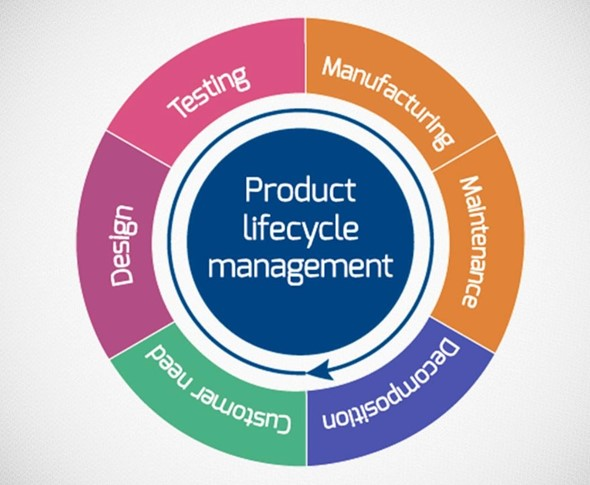
\includegraphics[width=15cm]{1}
\caption{\Large Product lifecycle stages產品生命週期階段}\label{fig.1}
\end{center}
\end{figure}
\newpage
\fontsize{14pt}{2.5pt}\sectionef 
{PLM is above all a connecting technology, not an individual technology islet or information processing system (Saaksvuori and Immonen, 2008). The idea is that every information produced by company personnel holds value equivalent to the time and money invested. Using that information saves money, not using that information wastes money. This is easier to understand when looking to a design process.}\\[1pt]

\fontsize{14pt}{5pt}\sectionef
 {PLM 首先是一種連結技術,而不是一個單獨的技術島或資訊處理系統(Saaksvuori 和 Immonen,2008)。 我們的想法是,公司人員產生的每個訊息都具有與投入的時間和金錢相當的價值。 使用該資訊可以節省金錢,而不使用該資訊會浪費金錢。 當查看設計過程時,這一點更容易理解。}\\[15pt]

\fontsize{14pt}{2.5pt}\sectionef 
{E.g. if an engineer designs an electronic circuit, the file holding the CAD drawing has an equivalent value to the time and money invested in it. The problem comes from the fact that in a traditional system only the engineer knows the design process behind the file, the extent of what is inside and its possible uses. While, from the perspective of the rest of the company, that is just a file in the database alongside thousands of others. The result is that, on its own, the information is of limited }\\[1pt]

\fontsize{14pt}{5pt}\sectionef
 {例如。 如果工程師設計電子電路,保存 CAD 圖紙的文件與投入的時間和金錢具有相同的價值。 問題在於,在傳統系統中,只有工程師知道文件背後的設計過程、內部內容的範圍及其可能的用途。 然而,從公司其他部門的角度來看,這只是資料庫中的一個文件,與數千個其他文件一起。 結果是,這些資訊本身的用途有限。}\\[15pt]

\fontsize{14pt}{2.5pt}\sectionef 
{If by any chance there is another engineer working in a similar design it will become extremely difficult for him/her to find that file and use it in his own design. Ultimately this results in waste because Engineer2 will have to spend more time and money doing something that wasalready made just because that information was not easily available or well organized. }\\[1pt]

\fontsize{14pt}{5pt}\sectionef
 {如果萬一有另一位工程師從事類似的設計,他/她將很難找到該文件並在自己的設計中使用它。 最終這會導致浪費,因為第二位工程師將不得不花費更多的時間和金錢來做一些已經完成的事情,因為這些資訊不容易獲得或組織良好。}\\[15pt]


\fontsize{14pt}{2.5pt}\sectionef 
{This scenario is not limited to product design, but also to all aspects of the product lifecycle that produces change over time. Someone had to orchestrate how that piece will be produced , how that piece will be moved,packed , distributed and disposed of. When a problem is found or improvements are possible those changes also produce information and consume resources. If the company cannot take advantage of that existing information about all those phases of the product conception it will waste resources at every single redesign.
}\\[1pt]

\fontsize{14pt}{5pt}\sectionef
 {這種場景不僅限於產品設計,還包括隨著時間的推移而產生變化的產品生命週期的各個方面。 必須有人精心策劃如何生產該作品,如何移動、包裝、分發和處置該作品。 當發現問題或可能進行改進時,這些變更也會產生資訊並消耗資源。 如果公司不能利用有關產品構思所有這些階段的現有信息,那麼每次重新設計都會浪費資源。}\\[15pt]
\newpage

\fontsize{14pt}{2.5pt}\sectionef 
{Product Lifecycle Management consists of an information system that allows information and knowledge sharing within and betweenorganizations (Sudarsan et al., 2005) minimizing the waste by controlling and organizing those files with information that would otherwise be carried only by the human resource that produced said files. The way it accomplishes that is by virtualizing all components of the product life-cycle in the form of digital “items” in an object oriented architecture. As explained by (Saaksvuori and Immonen, 2008),an item is a systematic and standard way to identify, encode and name a product, a product element or module, a component, a material or a service.
}\\[1pt]

\fontsize{14pt}{5pt}\sectionef
 {產品生命週期管理由一個資訊系統組成,該系統允許組織內部和組織之間共享資訊和知識(Sudarsan et al., 2005),透過控制和組織這些文件的資訊來最大限度地減少浪費,否則這些文件只能由產生所述文件的人力資源攜帶。 它實現這一目標的方式是在物件導向的架構中以數位「專案」的形式虛擬化產品生命週期的所有元件。 如(Saaksvuori 和 Immonen,2008)所解釋的,項目是識別、編碼和命名產品、產品元素或模組、組件、材料或服務的系統和標準方法。}\\[15pt]


\fontsize{14pt}{2.5pt}\sectionef 
{These item objects are, by all means, virtual representations that hold metadata regarding what it tries to represent and allows to connect and link the information. As described by (D’Antonio et al., 2015) product information should be connected to its production process. PLM allows to link defined processes to the product and to provide constraints on the order of process execution. E.g. a CAD drawing for a circuit schematic is attached to a virtual circuit object that holds basic information about what is contained in the file and all the previous iterations of that file over time as well as links to items representing which bill of materials (BOM) it belongs to, the machines necessary to manufacture it, the processes necessary to assemble it and more importantly how all those items changed over each improving iteration.
}\\[1pt]

\fontsize{14pt}{5pt}\sectionef
 {無論如何,這些項目物件都是虛擬表示,它們保存有關其試圖表示的內容的元數據,並允許連接和連結資訊。 如(D’Antonio 等人,2015)所述,產品資訊應與其生產過程相關聯。 PLM 允許將定義的流程連結到產品,並對流程執行的順序提供約束。 例如。 電路原理圖的 CAD 繪圖附加到虛擬電路對象,該對象保存有關文件中包含的內容以及該文件隨時間推移的所有先前迭代的基本信息,以及表示其物料清單 (BOM) 的項目的鏈接屬於,製造它所需的機器,組裝它所需的流程,更重要的是所有這些項目在每次改進迭代中如何變化。}\\[15pt]

\fontsize{14pt}{2.5pt}\sectionef 
{This all-around virtualization gives precious context to information otherwise lost on its own complexity. It allows for faster access, easier understanding of the whole and the consequences of what happens when there is change for each part. This is the best way of organizing the existing data for future reference because it allows for structure as well as transparency.
}\\[1pt]

\fontsize{14pt}{5pt}\sectionef
 {這種全方位的虛擬化為資訊提供了寶貴的背景信息,否則會因其自身的複雜性而丟失。 它允許更快地訪問、更容易理解整體以及每個部分發生變化時所發生的後果。 這是組織現有資料以供將來參考的最佳方式,因為它允許結構和透明度。}\\[15pt]
\newpage

\fontsize{14pt}{2.5pt}\sectionef 
{To sum up, PLM as a system aims to track functional change in all aspects regarding the product life, in a way that the company can benefit strategically from it by avoiding informational waste. It does so by virtualizing the real thing in the form of digital items that store the files regarding what the item is supposed to represent. These can in turn be correlated and tracked over time using metadata.
}\\[1pt]

\fontsize{14pt}{5pt}\sectionef
 {總而言之,PLM 作為一個系統,旨在追蹤產品生命週期各個方面的功能變化,從而使公司能夠透過避免資訊浪費來策略性地從中受益。 它透過以數位項目的形式虛擬化真實事物來實現這一點,這些項目儲存有關該項目應該代表的內容的文件。 這些又可以使用元資料隨著時間的推移進行關聯和追蹤。}\\[15pt]
\section{Enterprise Resource Planing 企業資源規劃}

\fontsize{14pt}{2.5pt}\sectionef 
{In the early days of information systems, one of the first systems to find wide implementation was the called MRP (Material Requirements Planning). Although not necessarily software based, this system wide implementation was a natural consequence of computing technology and it aimed to solve bottlenecks regarding the material supplying and product output by calculating the material needs for production. As it became more ubiquitous in the enterprise in the late 70’s and early 80’s the system evolved. This gave origin to MRP II (Manufacturing Resource Planning) and, more important to the scope of this paper, ERP (Enterprise Resource Planning).}

\fontsize{14pt}{5pt}\sectionef
 {在資訊系統的早期,最早被廣泛實施的系統之一是 MRP(物料需求計劃)。 儘管不一定基於軟體,但這種系統範圍的實施是計算技術的自然結果,旨在透過計算生產的材料需求來解決材料供應和產品輸出的瓶頸。 20 世紀 70 年代末和 80 年代初,隨著它在企業中變得越來越普遍,該系統也在不斷發展。 這催生了 MRP II(製造資源計劃),以及對本文範圍更重要的 ERP(企業資源計劃)。}\\[15pt]

\fontsize{14pt}{2.5pt}\sectionef 
{For the most part modern Enterprise Resource Planning expands the original MRP function to encompass many other aspects of enterprise operations all while adding modularity to the system. }

\fontsize{14pt}{5pt}\sectionef
 {現代企業資源規劃在很大程度上擴展了原始 MRP 功能,以涵蓋企業營運的許多其他方面,同時為系統添加了模組化功能。}\\[15pt]

\fontsize{14pt}{2.5pt}\sectionef 
{Modern ERP systems are often module based; different modules have different user interfaces and different user groups. For example, Manufacturing module, Procurement module, Logistics module, Financial module, Maintenance module, Sales module. (Saaksvuori and Immonen, 2008). These modules expand across many domains of knowledge but for the most part they do so always from the perspective of Production, Sales and Service. Figure 2 depicts the scope of the ERP system in comparison to other Information systems. }

\fontsize{14pt}{5pt}\sectionef
 {現代 ERP 系統通常是基於模組的; 不同的模組有不同的使用者介面和不同的使用者群組。 例如,製造模組、採購模組、物流模組、財務模組、維護模組、銷售模組。 (Saaksvuori 和 Immonen,2008)。 這些模組涵蓋了許多知識領域,但大多數情況下,它們總是從生產、銷售和服務的角度進行。 圖 2 描述了 ERP 系統與其他資訊系統相比的範圍。}\\[15pt]
\newpage
\begin{figure}[hbt!]
\begin{center}
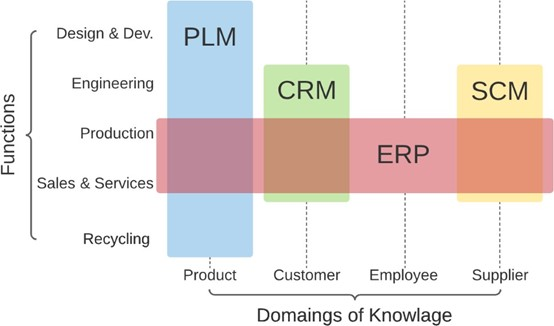
\includegraphics[width=15cm]{2}
\caption{\large Visual representation of the scope of different information systems不同資訊系統範圍的可視化表示}\label{fig.2}
\end{center}
\end{figure}

\fontsize{14pt}{2.5pt}\sectionef 
{This sort broad reach across the domains makes sense because the ERP operations, as were in the case of MRP, focus on handling transactions and orders. The focus of the ERP is controlling the change in input, retention and output of resources to the company, be of products, raw materials or packing. }

\fontsize{14pt}{5pt}\sectionef
 {這種跨領域的廣泛影響是有意義的,因為 ERP 操作與 MRP 一樣,專注於處理交易和訂單。 ERP 的重點在於控制公司資源(產品、原料或包裝)的輸入、保留和輸出的變化。}\\[15pt]

\fontsize{14pt}{2.5pt}\sectionef 
{From the same image, it is possible to see the theoretical contrast between PLM and ERP even though they are both extremely broad. While ERP expands across the domains of knowledge but limits itself to a few functions, PLM expands across all functions that involve the product. As portrayed by Figure 3, another point of view that represents a good difference between the two is the lack of overlap in what concerns the scale or level of detail in which ERP and PLM affects the industry (i.e. the granularity of the two systems).}

\fontsize{14pt}{5pt}\sectionef
 {從同一張圖中,可以看出 PLM 和 ERP 之間的理論差異,儘管它們的範圍都非常廣泛。 ERP 擴展了知識領域,但僅限於少數功能,而 PLM 擴展了涉及產品的所有功能。 如圖 3 所示,代表兩者之間良好差異的另一個觀點是 ERP 和 PLM 影響行業的規模或詳細程度(即兩個系統的粒度)方面缺乏重疊。}\\[15pt]
\newpage

\begin{figure}[hbt!]
\begin{center}
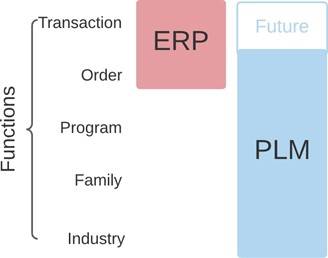
\includegraphics[width=15cm]{3}
\caption{\large Visual comparison of ERP and PLM concerning granularity ERP 和 PLM 在粒度方面的直觀比較}\label{fig.3}
\end{center}
\end{figure}

\fontsize{14pt}{2.5pt}\sectionef 
{As we can see, ERP is primarily concerned with the transaction and the order. Once an order is closed out, the ERP system processes the transactions with respect to that order but is not very much concerned with the order beyond that. On the other hand, PLM’s granularity is concerned with the order for the product and extends not only into the program, but into 
the family and the entire industry .}

\fontsize{14pt}{5pt}\sectionef
 {正如我們所看到的,ERP 主要關注的是交易和訂單。 一旦訂單關閉,ERP 系統就會處理與該訂單相關的交易,但不太關心除此之外的訂單。 另一方面,PLM 的粒度涉及產品的訂單,不僅擴展到程序,還擴展到
家庭和整個行業。}\\[15pt]
\newpage
\fontsize{14pt}{2.5pt}\sectionef 
{This is particularly interesting because it demonstrates how the two systems can and do complement each other in the field. One of the aspects of ERP that should point out is that it is comparatively easier to integrate with other systems. ERP-MES integration for instance has been widely studied and implemented to the point where standards have been developed for it (ISA 95 - IEC 62264). One argument for this is the modular nature of the ERP system which is discussed further in the paper in (Chapter 5) with the analysis of the Odoo software. That is because the Odoo software evolved originally from an open-source ERP system.}

\fontsize{14pt}{5pt}\sectionef
 {這是特別有趣的,因為它展示了這兩個系統如何能夠並且確實在該領域中相互補充。 ERP值得指出的一方面是它與其他系統的整合相對容易。 例如,ERP-MES 整合已被廣泛研究和實施,並已為其製定了標準(ISA 95 - IEC 62264)。 對此的一個論點是 ERP 系統的模組化性質,這將在本文(第 5 章)中透過對 Odoo 軟體的分析進行進一步討論。 這是因為 Odoo 軟體最初是從開源 ERP 系統發展而來的。}\\[15pt]

\fontsize{14pt}{2.5pt}\sectionef 
{The nature of the ERP system is best summed up by (Umble et al. 2003): ERP provides a unified enterprise view of the business which encompasses all functions and departments, and an enterprise database in which all actions concerning finance, sales, marketing, purchasing and human resources are traced. The aim of this achieving is to expand the customers target and increase customers share in a market that slowly pivots to innovation .
}

\fontsize{14pt}{5pt}\sectionef
 {ERP 系統的本質可以這樣概括(Umble et al. 2003):ERP 提供了一個統一的企業業務視圖,其中包含所有職能和部門,以及一個企業資料庫,其中涉及財務、銷售、行銷、採購和人力資源都被追蹤。 實現這一目標的目的是擴大客戶目標並增加緩慢轉向創新的市場中的客戶份額。}\\[15pt]
\section{Manufacturing Execution System 製造執行系統}


\fontsize{14pt}{2.5pt}\sectionef 
{The final key of a fully integrated system would be the Manufacturing Execution System (MES). A MES is a layer of communication between  he management and the production levels; it is a software that allows data exchange between the organizational level, usually supported by an ERP, and the shop-floor control systems, in which several, different, very customized software applications are employed (Meyer et al., 2009).}

\fontsize{14pt}{5pt}\sectionef
 {完全整合系統的最後一個關鍵是製造執行系統(MES)。 MES 是管理階層與生產層之間的溝通層; 它是一種允許組織層面(通常由 ERP 支援)和車間控制系統之間進行資料交換的軟體,其中使用了多種不同的、高度客製化的軟體應用程式(Meyer 等人,2009 年)。}\\[15pt]

\fontsize{14pt}{2.5pt}\sectionef 
{Figure 4 is a nice depiction of how different systems fit within the scope of manufacturing and development.}

\fontsize{14pt}{5pt}\sectionef
 {圖 4 很好地描述了不同的系統如何適應製造和開發的範圍。}\\[15pt]
\newpage

\begin{figure}[hbt!]
\begin{center}
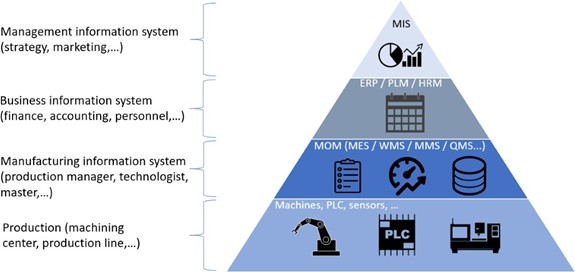
\includegraphics[width=15cm]{4}
\caption{\small Visual representation of the roll of different systems including MES\\
 包括 MES 在內的不同系統的滾動視覺化表示}\label{fig.4}
\end{center}
\end{figure}

\fontsize{14pt}{2.5pt}\sectionef 
{For all purposes MES main goal is to provide the numbers and data that ultimately is used to ascertain the condition and quality of not only the products but also all the processes that affect production. Machines, sensors, and anything that comes in contact with the product and provides output of any kind, basically, handing said data to the MES for sorting and processing in real time. E.g. if a manager wants to know the instant production numbers or to see a graphical representation of the rejection rate, that data will be available from a MES software.}

\fontsize{14pt}{5pt}\sectionef
 {出於所有目的,MES 的主要目標是提供最終用於確定產品以及影響生產的所有流程的狀況和品質的數字和數據。 機器、感測器以及與產品接觸並提供任何類型輸出的任何東西,基本上將所述資料傳遞給 MES 進行即時分類和處理。 例如。 如果經理想要了解即時生產數據或查看廢品率的圖形表示,則可以從 MES 軟體取得該數據。}\\[15pt]

\fontsize{14pt}{2.5pt}\sectionef 
{Traditionally it is from this sort of information that management will evaluate efforts and make decisions. As mentioned before this sort of data collection fits perfectly to the use of ERP not only because the management of resources can be much more detailed if complemented by real time production data but also because the modularity of ERP usually means a seamless integration. MES (like ERP) has also been proven and implemented for decades and their implementation have already been standardized to a reasonable degree.
}

\fontsize{14pt}{5pt}\sectionef
 {傳統上,管理層將根據此類資訊評估工作並做出決策。 如前所述,這種數據收集非常適合 ERP 的使用,不僅因為如果輔以即時生產數據,資源管理可以更加詳細,而且還因為 ERP 的模組化通常意味著無縫整合。 MES(如 ERP)也已被證明和實施了數十年,其實施已達到合理的標準化程度。}\\[15pt]
\newpage



\fontsize{14pt}{2.5pt}\sectionef 
{The functionalities of a MES have been grouped in 11 categories by MESA International(1997); furthermore, the tasks for each enterprise layer and, in turn, for each kind of information system are listed in the ISA95 – IEC62264 (2013) standard. This standard also provides definitions for the data structures to be exchanged among information systems aiming to enhance their integration; however, it mainly focuses on ERP-MES-Shop floor integration (D’Antonio et al., 2015).
}

\fontsize{14pt}{5pt}\sectionef
 {MESA International (1997) 將 MES 的功能分為 11 類; 此外,ISA95 – IEC62264 (2013) 標準中列出了每個企業層以及每種資訊系統的任務。 該標準還提供了資訊系統之間交換的資料結構的定義,旨在增強資訊系統的整合度; 然而,它主要關注 ERP-MES-車間整合(D’Antonio 等,2015)。}\\[15pt]


\fontsize{14pt}{2.5pt}\sectionef 
{PLM studies by comparison are much more recent and PLM-MES integration, a main focus of this work, even more so. The challenge of this sort of integration and the state of the art regarding it was be covered in (Chapter 3) as well as the theoretical structure behind it. For now, suffice to point out that since MES provides the feedback by which changes are orchestrated and results are validated by generating information in the form of files and PLM focus on the tracking change by file organization there sure is value in the PLM-MES 

}

\fontsize{14pt}{5pt}\sectionef
 {相較之下,PLM 研究是較新的,而 PLM-MES 整合(這項工作的主要焦點)更是如此。 (第 3 章)及其背後的理論結構涵蓋了這種整合的挑戰和相關的最新技術。 目前,只需指出,由於 MES 提供回饋,透過產生文件形式的資訊來編排變更並驗證結果,而 PLM 專注於按文件組織追蹤變更,因此 PLM-MES 確實有價值
一體化。}\\[15pt]

\section{Industry 4.0 工業4.0}

\fontsize{14pt}{2.5pt}\sectionef 
{The term Industry 4.0 is one mentioned time and time again in modern literature as the next or current step in the evolution of production. It represents what is the 4th industrial revolution where the first was marked the adoption of steam power, the second was marked mainly using electrical power and the 3rd was characterized by the implementation of digital technology. Figure 5 nicely represents the progression of industrial revolutions.


}

\fontsize{14pt}{5pt}\sectionef
 {工業 4.0 一詞在現代文獻中被多次提及,被視為生產演變的下一步或當前步驟。 它代表了第四次工業革命,第一次工業革命的特徵是蒸汽動力的採用,第二次工業革命的特徵是主要使用電力,第三次工業革命的特徵是數位技術的實施。 圖 5 很好地展示了工業革命的進展。}\\[15pt]
\newpage
\begin{figure}[hbt!]
\begin{center}
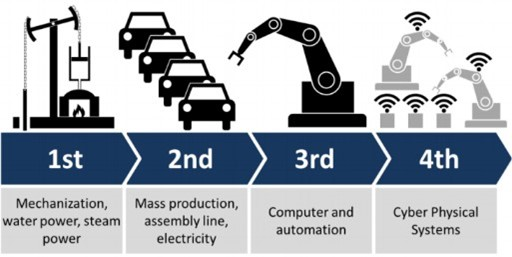
\includegraphics[width=15cm]{5}
\caption{\large The industry evolution產業演變}\label{fig.5}
\end{center}
\end{figure}


\fontsize{14pt}{2.5pt}\sectionef 
{In broad strokes the 4th industrial revolution is (or will be) ultimately marked by the full integration between digital connectivity and production. As it is well known that the development of digital networks is the pivotal technology that sustain the modern world. It has changed the way humans interact and do business. However, whether the current level in which it is applied to the industry constitutes an industrial revolution is still uncertain because in all other revolutions have been marked by a violent increase in production that is yet to happen this time around. In fact, we are still to reach a shared definition of Industry 4.0.
}

\fontsize{14pt}{5pt}\sectionef
 {從廣義上講,第四次工業革命的最終標誌是(或將)數位連接與生產之間的全面整合。 眾所周知,數位網路的發展是維持現代世界的關鍵技術。 它改變了人類互動和開展業務的方式。 然而,目前它應用於工業的水平是否構成工業革命仍然不確定,因為在所有其他革命中,其標誌都是產量的劇烈增加,而這一次尚未發生。 事實上,我們仍然沒有對工業4.0達成共同的定義。}\\[15pt]

\fontsize{14pt}{2.5pt}\sectionef 
{What has been widely accepted however is that there are at least 3 technologies that characterize Industry 4.0. Those are the Internet of things (IoT), Cloud computing and the development of Cyber-Physical Systems (CPS), the last of which is particularly important for the context of this thesis.}

\fontsize{14pt}{5pt}\sectionef
 {然而,人們普遍認為至少有 3 種技術可以表徵工業 4.0。 這些是物聯網(IoT)、雲端運算和網路物理系統(CPS)的發展,最後一個對於本論文的背景尤其重要。}\\[15pt]

\newpage



\fontsize{14pt}{2.5pt}\sectionef 
{CPS are systems consisting in a real entity (for example, a machine) and its corresponding virtual model – embedding all the models for mimicking the behavior of the real counterpart – capable to communicate with each other (D’Antonio et al., 2017). The idea is that, if one were to develop a digital twin (DT) of all physical instruments regarding a process in a system that allows for the digital counterparts to interact with each other as well as interacting with the physical world, innovation or change of said process would occur much faster and effectively. E.g., an engineer could simulate a change using the DT’s interaction, then, if successful, apply the change automatically to the production line in real time, execute tests, gather data and feed it back to the system without the need of manual input with all being done through the network.}

\fontsize{14pt}{5pt}\sectionef
 {CPS 是由真實實體(例如機器)及其相應的虛擬模型組成的系統 - 嵌入所有用於模仿真實對應物行為的模型 - 能夠相互通信(D'Antonio 等人,2017) 。 這個想法是,如果要開發所有實體儀器的數位孿生(DT),涉及系統中的一個過程,允許數位對應物相互交互以及與物理世界交互,創新或改變該過程將發生得更快、更有效。 例如,工程師可以使用DT的交互來模擬變更,然後,如果成功,則將變更自動即時應用到生產線,執行測試,收集數據並將其反饋給系統,而無需手動輸入所有內容是透過網路完成的。}\\[15pt]

\fontsize{14pt}{2.5pt}\sectionef 
{The main point to be derived from all this is that PLM-MES systems possibly are the first step to achieve a proper CPS since it provides for the virtualization and necessary control to reach something near a virtual twin. The debatable matter is how deep is its current effect in industrial application.}

\fontsize{14pt}{5pt}\sectionef
 {從這一切中得出的要點是,PLM-MES 系統可能是實現適當 CPS 的第一步,因為它提供了虛擬化和必要的控制來達到接近虛擬孿生的效果。 值得爭議的問題是它目前在工業應用中的影響有多深。}\\[15pt]

\fontsize{14pt}{2.5pt}\sectionef 
{Nonetheless, the term Industry 4.0 is, if anything, a useful denotation to the increasing application of digital connectivity, network development and the internet to industry.}

\fontsize{14pt}{5pt}\sectionef
 {儘管如此,工業 4.0 這個術語如果有的話,也是對數位連接、網路發展和互聯網在工業中日益增長的應用的有用表示。}\\[15pt]

\fontsize{14pt}{2.5pt}\sectionef 
{Another term often included within the scope of Industry 4.0 is the called Lot Size One or Lot 1. This is the idea of each item customized to the individual specifications of the buyer in a system in which a customer order does not start supply chain equipment moving; it turns on manufacturing machines.}

\fontsize{14pt}{5pt}\sectionef
 {工業4.0 範圍內經常包含的另一個術語稱為“批量大小一”或“批量1”。這是在系統中根據買方的個人規格定制每個項目的想法,在該系統中,客戶訂單不會啟動供應鏈設備移動; 它打開製造機器。}\\[15pt]
\newpage

\fontsize{14pt}{2.5pt}\sectionef 
{The theory behind it is that as production and development becomes more and more flexible as this sort of manufacturing becomes not only viable but also attractive. Having a tailored requested product means that there are no storage requirements, no inventory overhead, and of course a 100percent guaranteed sell. This concept is not new by any means, in fact it predates Industry 4.0 quite a lot. In the book “The machine that changed the world”the authors (Womack et al., 1990) discuss that toward this end, lean producers employ teams of multiskilled workers at all levels of the organization and use highly flexible, increasingly automated machines to produce volumes of products in enormous variety.}

\fontsize{14pt}{5pt}\sectionef
 {背後的理論是,隨著生產和開發變得越來越靈活,這種製造不僅變得可行而且有吸引力。 擁有量身訂製的需求產品意味著沒有儲存要求、沒有庫存開銷,當然還有 100percent 的銷售保證。 無論如何,這個概念並不新鮮,事實上它早在工業 4.0 之前就出現了。 在《改變世界的機器》一書中,作者(Womack 等人,1990)討論了為此目的,精益生產者在組織的各個層面僱用多技能工人團隊,並使用高度靈活、自動化程度越來越高的機器來生產大量種類繁多的產品。}\\[15pt]

\fontsize{14pt}{2.5pt}\sectionef 
{In a way ‘Lot Size One’ is nothing more than the extrapolation of this sort of thinking. Of course, the industry is yet to reach such level of production flexibility, but glimpses of this sort of mentality can already be seem on more modular productions. One of the best examples is amazon packing systems. E.g. a customer receives a package from Amazon containing a mix of products that has been packaged just for him/her according to their specific order. Although superficial in nature, this represents a high level of customization for the customer. }

\fontsize{14pt}{5pt}\sectionef
 {在某種程度上,「批量一」只不過是這種思考的推論。 當然,該行業尚未達到這樣的生產靈活性水平,但這種心態已經可以在更模組化的生產中看到。 最好的例子之一是亞馬遜包裝系統。 例如。 客戶收到亞馬遜的包裹,其中包含根據其特定訂單專門為他/她包裝的產品組合。 雖然本質上很膚淺,但這代表了客戶的高水準客製化。}\\[15pt]

\fontsize{14pt}{2.5pt}\sectionef 
{Another great example is electronics prototyping. Currently there are companies that take your printed circuit board designs and BOM, delivering small batches of assembled prototypes at a low cost. Prototyping of electronical devices used to be a highly expensive process, but some companies have flexibilized their production to the degree where they are able to deliver it fast and reliably. Again, that is possible because electronics components are inherently modular systems even if of high complexity. The following image (Figure 6 Example project of power supply adaptor circuit) is an example of an electronic circuit that was designed by this student and manufactured by JLCPCB within a single week.}

\fontsize{14pt}{5pt}\sectionef
 {另一個很好的例子是電子原型設計。 目前,有些公司會採用您的印刷電路板設計和 BOM,以低成本提供小批量的組裝原型。 電子設備的原型設計曾經是一個非常昂貴的過程,但一些公司已經將其生產靈活化到能夠快速可靠地交付的程度。 同樣,這是可能的,因為電子元件本質上是模組化系統,即使其複雜性很高。 下圖(圖6電源適配器電路範例專案)是該學生設計並由JLCPCB在一週內製造的電子電路範例。}\\[15pt]
\newpage

\begin{figure}[hbt!]
\begin{center}
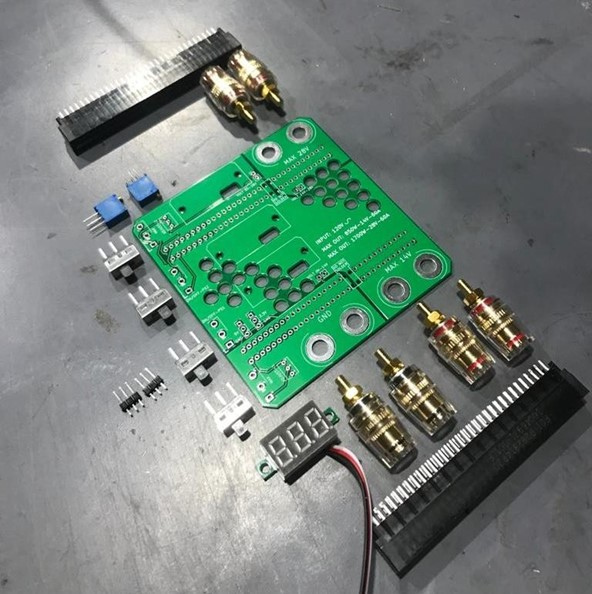
\includegraphics[width=15cm]{6}
\caption{\large Example project of power supply adaptor circuit\\電源適配器電路範例項目}\label{fig.6}
\end{center}
\end{figure}

\fontsize{14pt}{2.5pt}\sectionef 
{All and all, the result is again a greater need for control and management of change. Which means the implementation of a PLM-MES system would be of great help. PLM would be required to manage change and innovation throughout the lifecycle of small batch products and MES would provide the real time reaction and feedback necessary to reduce errors that could cause losing a whole batch.
}

\fontsize{14pt}{5pt}\sectionef
 {總而言之,結果再次是對變革的控制和管理的更大需求。 這意味著PLM-MES系統的實施將會有很大的幫助。 PLM 需要在小批量產品的整個生命週期中管理變更和創新,而 MES 將提供必要的即時反應和回饋,以減少可能導致整批產品遺失的錯誤。}\\[15pt]
\newpage
\end{document}